%---------------------------------------
\section{VELOCIDAD DE AVANCE DE ONDAS DE PEQUEÑA AMPLITUD} \label{sec:velocidad_pequena}
%---------------------------------------
Para cuantificar la velocidad de avance generada por el movimiento de onda viajera descrito, en primer lugar se describirán las ecuaciones diferenciales propuestas en \cite{Gray1955} para su cálculo. Posteriormente se verificará la precisión del método mediante las expresiones teóricas calculadas anteriormente y finalmente se determinará la velocidad para la nueva expresión de onda viajera propuesta (\ref{eq:flag_fish_traveling_wave_fractional}).
\begin{figure}[!h] %  figure placement: here, top, bottom, or page
	\vspace*{3mm}
    \centering
    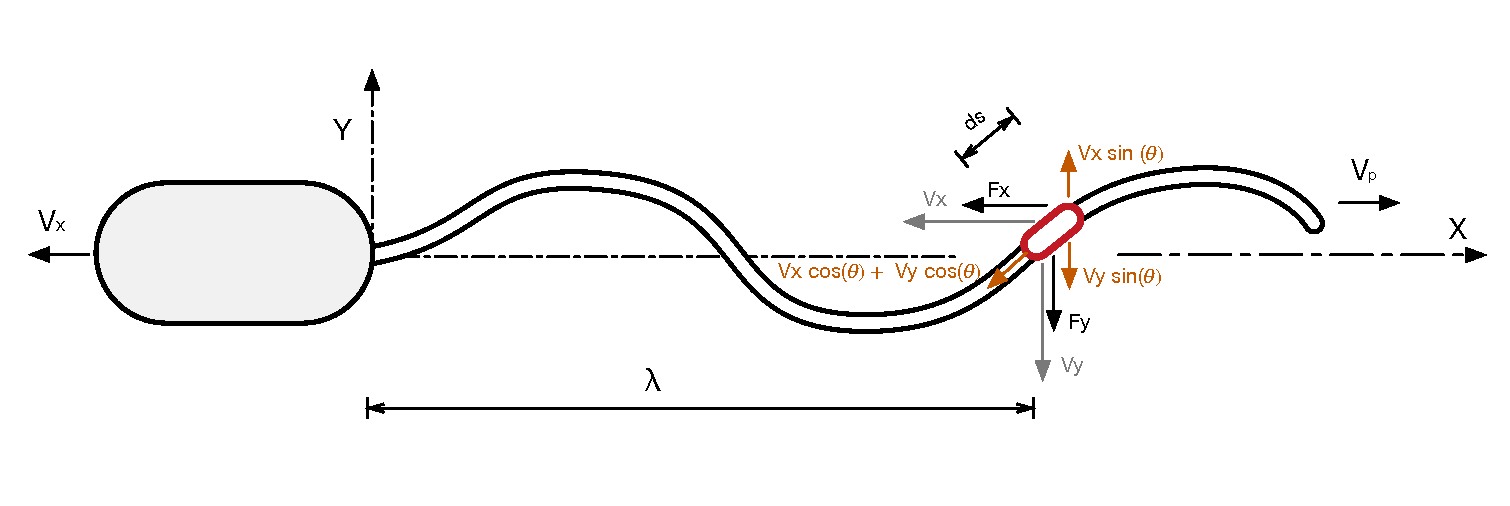
\includegraphics[width=0.9\textwidth]{Figuras/flagelo_dx}
  	\caption{Sólido libre de un elemento infinitesimal del flagelo.}
  	\label{fig:solido_flag}
\end{figure}

De acuerdo al planteamiento y análisis descrito en \cite{Gray1955} la velocidad lograda es debido a la fuerza de propulsión generada por el flagelo. Siendo la fuerza ejercida por un elemento infinitesimal del flagelo 
\begin{eqnarray}
	\label{eq:dF_ds}
	\frac{dF}{ds}= \frac{(C_N - C_L) \frac{dy}{dt}\frac{dy}{dx} - V_x \left(  C_L + C_N \frac{dy}{dx} ^2 \right)}{1 + \frac{dy}{dx}^2},
\end{eqnarray}
donde $y(x,t)$ define la forma de onda, $C_N$ y $C_L$ representan el coeficiente de rozamiento normal y tangencial, $V_x$ es la velocidad de avance, $\frac{dy}{dt}$ es la velocidad transversal y $\frac{dy}{dx}$ el ángulo de inclinación del elemento considerado respecto al eje de desplazamiento. Suponiendo unas dimensiones y oscilaciones relativamente pequeñas, es posible aproximar el diferencial de superficie por un diferencial de longitud ($ds \approx dx$) y despreciar los términos de segundo orden. Así pues, es posible conocer la velocidad de avance afirmando que la fuerza de propulsión total para una oscilación completa es igual a la fuerza necesaria para vencer la fuerza de arrastre debida al cuerpo, descrita como:
\begin{eqnarray}
	\label{eq:dF=}
	nF = C_C V_x
\end{eqnarray}
donde $n$ es el número oscilaciones simultáneas que recorren el flagelo y $C_C$ representa el coeficiente de arrastre de la cabeza, que para una esfera de radio $R$ viene dado por la expresión
\begin{equation}
C_C=6 \pi \mu R.
\end{equation}
\

Respecto las derivadas respecto del tiempo y el espacio de las ecuaciones definidas anteriormente (\ref{eq:flag_fish_traveling_wave}) y (\ref{eq:flag_fish_traveling_wave_fractional}) son:
\begin{eqnarray}
	\label{eq:dy_dt}
	\frac{dy}{dt} = - \frac{2 \pi V_p}{\lambda}  (c_0 + c_1 x^{\alpha} + c_2 x^2) \cos \left( \frac{2 \pi}{\lambda}  ( x - V_p t) \right), 
\end{eqnarray}
\begin{eqnarray}
	\label{eq:dy_dx}
		\frac{dy}{dx} = \frac{2 \pi }{\lambda}  (c_0 + c_1 x^{\alpha} + c_2 x^2) \cos \left( \frac{2 \pi}{\lambda}  ( x - V_p t) \right)\\
		 + (\alpha c_1 x^{\alpha-1} + 2 c_2 x) \sin \left(  \frac{2 \pi}{\lambda}  ( x - V_p t) \right), \nonumber
\end{eqnarray}

términos que representan la principal complejidad para su integración numérica y algebraica. Además de ser los principales componentes que determinan la fuerza de propulsión.\\

Después de varias cálculos y simplificaciones, es posible presentar la velocidad de avance como la siguiente ecuación diferencial:
\begin{eqnarray}
\label{eq:Vx_dx}
	\frac{V_x (t)}{dx} =  \left( \frac{C_N - C_L}{C_L} \right) \left( \frac{1}{ n \lambda + \frac{6 \pi R \mu}{C_L} }  \right) \frac{dy}{dt} \frac{dy}{dx}.
	\end{eqnarray}

%---------------------------------------
\subsection{Descripción del script de integración numérica} \label{sec:descripcion_script}
%-------------------------------------
Para implementar el script de integración numérica la ecuación anterior han sido agrupada en diversos términos como se muestra en la siguiente Figura:
\begin{figure}[!h] %  figure placement: here, top, bottom, or page
	\vspace*{3mm}
    \centering
    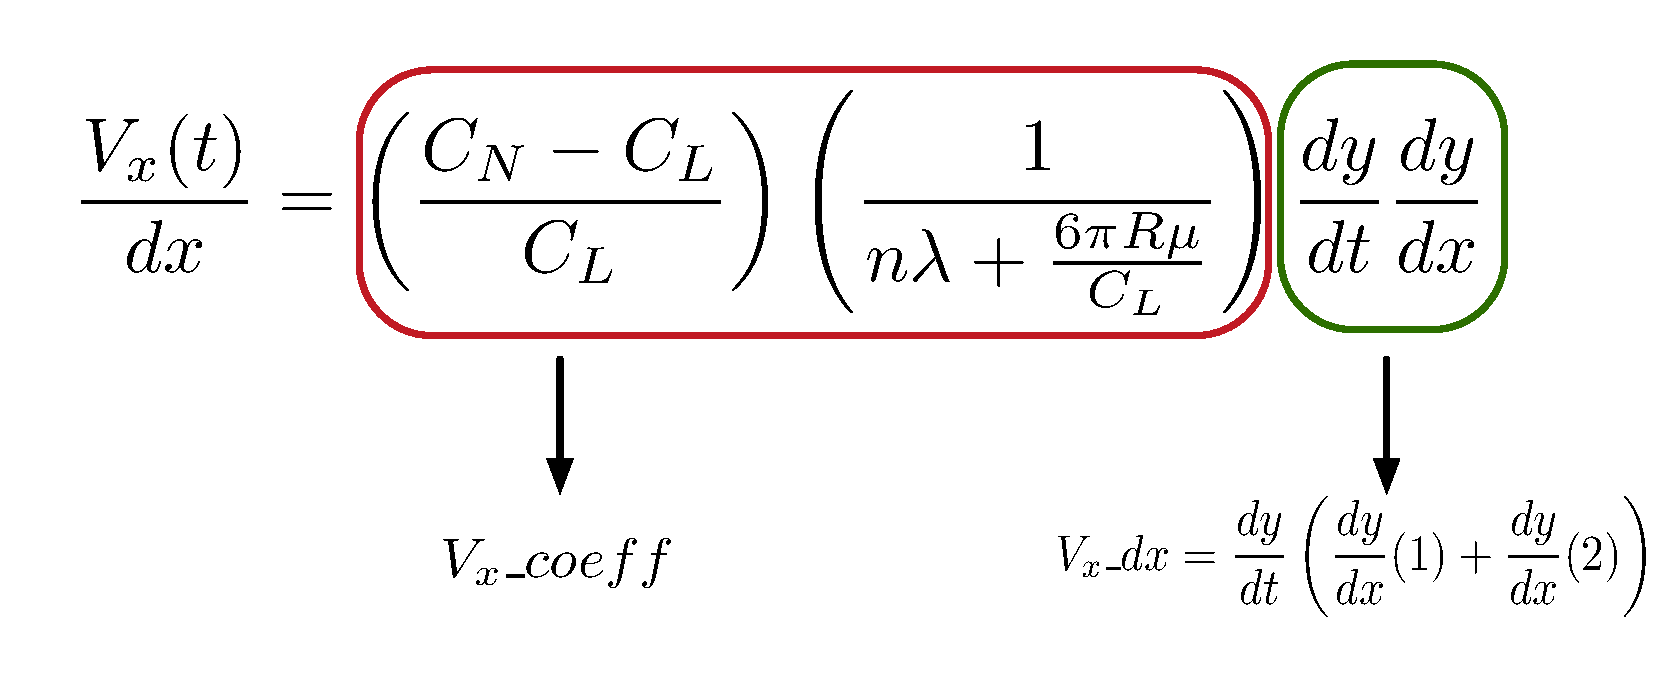
\includegraphics[width=0.6\textwidth]{Figuras/FDF}
  	\caption{Agrupación de términos.}
  	\label{fig:OVF}
\end{figure}

donde $V_{x}\_coeff$ es un término constante, y $V_x\_dx$ representa el producto de las derivadas indicadas anteriormente (\ref{eq:dy_dt}) y (\ref{eq:dy_dx}), las cuales son dependientes del tiempo y el espacio. Además, la derivada respecto al espacio ha sido separada en sus dos sumandos principales para una mejor compresión del código desarrollado.\\

Respecto a las funciones diferenciales han sido definidas como funciones paramétricas dependientes de la coordenada en el espacio, para cada instante de tiempo. Siendo necesario un bucle de interacción que calcule la velocidad de avance en cada instante de tiempo, obteniendo así un array de velocidades. A continuación se muestra el fragmento del script donde se obtiene el valor de la velocidad.
\begin{lstlisting}[]
%% Calculo de la velocidad de avance por integración numérica.

% Vx = (n * (CN - CL)) / (Cc + n * lambda * CL) * ( dy / dt * dy/dx dx)
% Vx = |------------- vx_coeff ---------------| * |------ vx_dx -------|
%                                         |-- dy_dt * (dy_dx1 + dy_dx2) --|

vx_coeff = ( (1/lambda) * (CN - CL) / CL )...
            * ( 1 / (1 + Cc/ ( n * lambda * CL) ) ) ;

for i=1:length(t);
  
    dy_dt =@(x) -(2*pi*Vp/lambda) * (c0 + c1.*x.^alfa  + c2.*x.^2)...
                .* cos( (2*pi/lambda) * (x - Vp*t(i)) );

    dy_dx1 =@(x) (2*pi/lambda) .* (c0 + c1.*x.^alfa + c2.*x.^2)...
                .* cos( (2*pi/lambda) * (x - Vp.*t(i)) );
    
    dy_dx2 =@(x) (2*c2.*x + alfa.*c1.*x.^(alfa-1))...
                .* sin( (2*pi/lambda) * (x - Vp.*t(i)) ); 
        
    vx_dx =@(x) dy_dt(x) .* (dy_dx1(x) + dy_dx2(x));                                     
   	
   	% Función de integración numérica -- quadgk
    % Numerically evaluate integral, adaptive Gauss-Kronrod quadrature.
    NVx = [NVx  quadgk(vx_dx,0,lambda)];
end
                                
NVx = NVx .* vx_coeff;

\end{lstlisting}
\

La función utilizada para realizar concretamente la integración numérica es la indicada en el extracto anterior del script ``\textbf{quadgk}''. Función que emplea un algoritmo de cálculo basado en la cuadratura adaptativa de Gauss-Kronrod. Respecto a su parámetros de configuración se han utilizados los definidos por defecto, es decir, una tolerancia absoluta de $10^{-10}$ y relativa de $10^{-6}$ para variables de tipo \textit{double}.

%---------------------------------------
\subsection{Verificación y validación del algoritmo de integración numérica} \label{sec:verificacion_script}
%-------------------------------------

Una vez desarrollado el script el siguiente paso es verificar que los resultados ofrecidos por la función de cálculo numérico son válidos en comparación a valores conocido. Por ello, en primer lugar se calculara la velocidad para la expresión de onda viajera (\ref{eq:flag_fish_traveling_wave}), cuya velocidad teórica conocida a través de (\ref{eq:Vx_fish}). Aunque previamente es necesario indicar cuales serán el valor numérico de los parámetros que serán usados, los cuales se exponen en la Tabla \ref{Tab:data_flagellum}.\\
\begin{table}[!h]
\centering
\caption{Valor de los parámetros, extraídos de \cite{Gray1955}}
\resizebox{0.9\textwidth}{!}{
\begin{tabular}{| c | c | c |}
  \hline
\cellcolor{lightgray} \textbf{Parámetros} & \cellcolor{lightgray} 
 \textbf{Expresión/Valor} & \cellcolor{lightgray} \textbf{Descripción} \\
 	\hline
$c_0$		& $4 \cdot 10^{-6}$ (m) & Amplitud máxima de las ondas. \\	
	\hline
$f$		& 35 (Hz) & Frecuencia de propagación.\\	
	\hline	
$\lambda$ & $24 \cdot 10^{-6}$  (m) & Longitud de onda de la onda viajera.	\\
	\hline
$n$ & $3$ & Numero de ondas simultáneas en el flagelo.	\\
	\hline
$R$ &  $5 \cdot 10^{-7}$ (m) & Radio de la cabeza. \\
	\hline
$d$ & $ 2 \cdot 10^{-7}$ (m)  & Radio del flagelo. \\
	\hline
$C_L$	& $\frac{2 \pi \mu }{ \log{\frac{d}{2 \lambda}} + \frac{1}{2}}$ & Coeficiente de arrastre tangencial. \\
	\hline
$C_N$	& $C_N = 2 C_L$ & Coeficiente de arrastre normal.\\
	\hline	
$C_C$	& 6$\pi$$\mu$$R$ & Coeficiente de arrastre de la cabeza.\\
  \hline
$\mu$ & $7^{-4}$ (Pa $\cdot$ s) & Viscosidad	 \cite{Majumdar2009}.	\\
	\hline		
\end{tabular}
\label{Tab:data_flagellum}
}
\end{table}

Una vez conocidos los datos, es posible verificar los resultados teóricos y numéricos obtenidos para diferentes magnitudes de los coeficientes de amplitud. Dichos coeficientes han sido seleccionados de forma que permitan alcanzar la amplitud máxima al final de una longitud de onda del flagelo, como se puede observar en la Figura \ref{fig:OVV}, donde el color azul representa la onda armónica, el verde la onda viajera de crecimiento lineal, y el color rojo identifica la onda viajera cuyo crecimiento es modulado con el coeficiente $c_2$.\\
\begin{figure}[!h] %  figure placement: here, top, bottom, or page
	\vspace*{3mm}
    \centering
    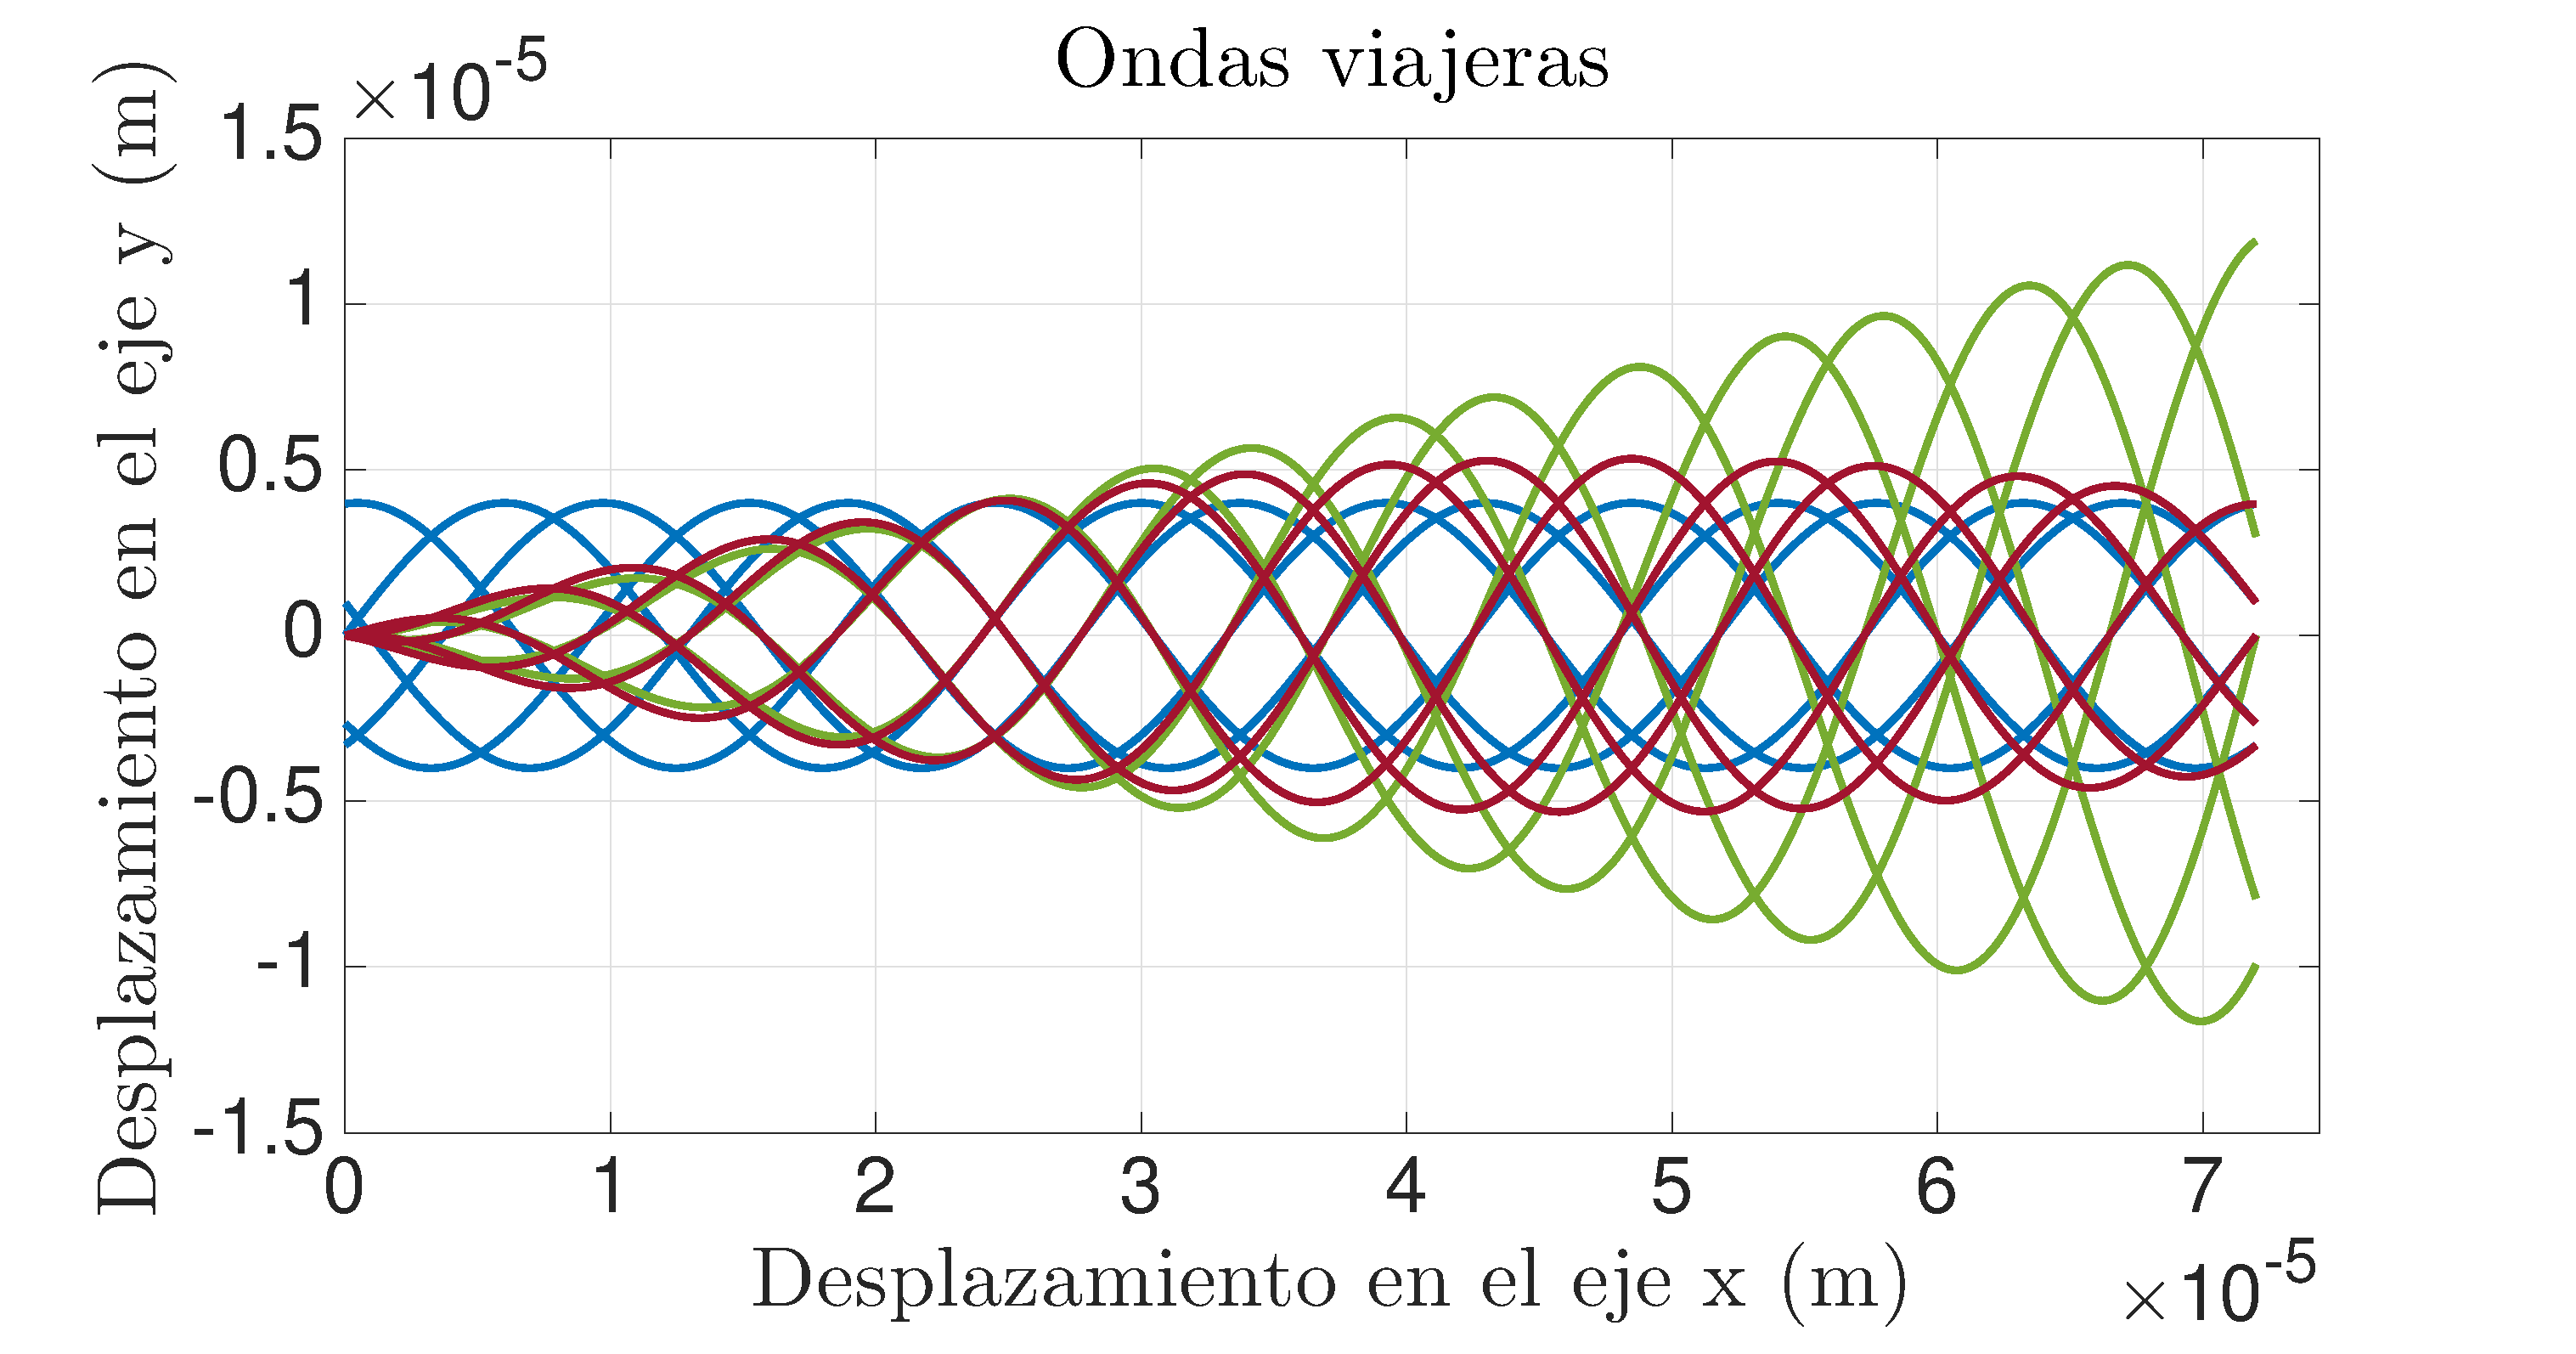
\includegraphics[width=0.9\textwidth]{Figuras/OVV}
  	\caption{Representación de las ondas viajeras empleadas para la verificación.}
  	\label{fig:OVV}
\end{figure}

De acuerdo al criterio de crecimiento en una longitud de onda el coeficiente $c_1$ se encuentran definido para la siguiente expresión
\begin{eqnarray}
	\label{eq:coeff_c1}
	c_1 = \frac{c_0}{n\lambda}.
\end{eqnarray}

Por otro lado, la combinación de los coeficientes $c_1$ y $c_2$ son definidos por (\ref{eq:coeff_c1yc2}), donde $m$ es un múltiplo de $\lambda$ y cumple la condición $m > n$.
\begin{eqnarray}
	\label{eq:coeff_c1yc2}
	c_1 &=& \frac{c_0 }{n \lambda} + \frac{m}{m - n}  \left( \frac{c_0} {m  \lambda} - \frac{n A} {m  \lambda} \right)\\
	c_2 &=& \frac{m}{m - n}  \left( \frac{A} {m  \lambda^2} - \frac{c_0} {n m  \lambda^2} \right) \nonumber
\end{eqnarray}

Finalmente los resultados obtenidos se muestran en la Figura \ref{fig:OVV}, lo cuales aprueban la validez del algoritmo y la función para calcular la velocidad de avance del movimiento de onda viajera por integración numérica. En dichos resultados se puede observar que tanto el valor obtenido por la función teórica (\ref{eq:Vx_fish}) e integración numérica coinciden con un RMSE de $ 2 \cdot 10^{-19}$ \% aproximadamente.
\begin{figure}[t] %  figure placement: here, top, bottom, or page
	\vspace*{3mm}
    \centering
    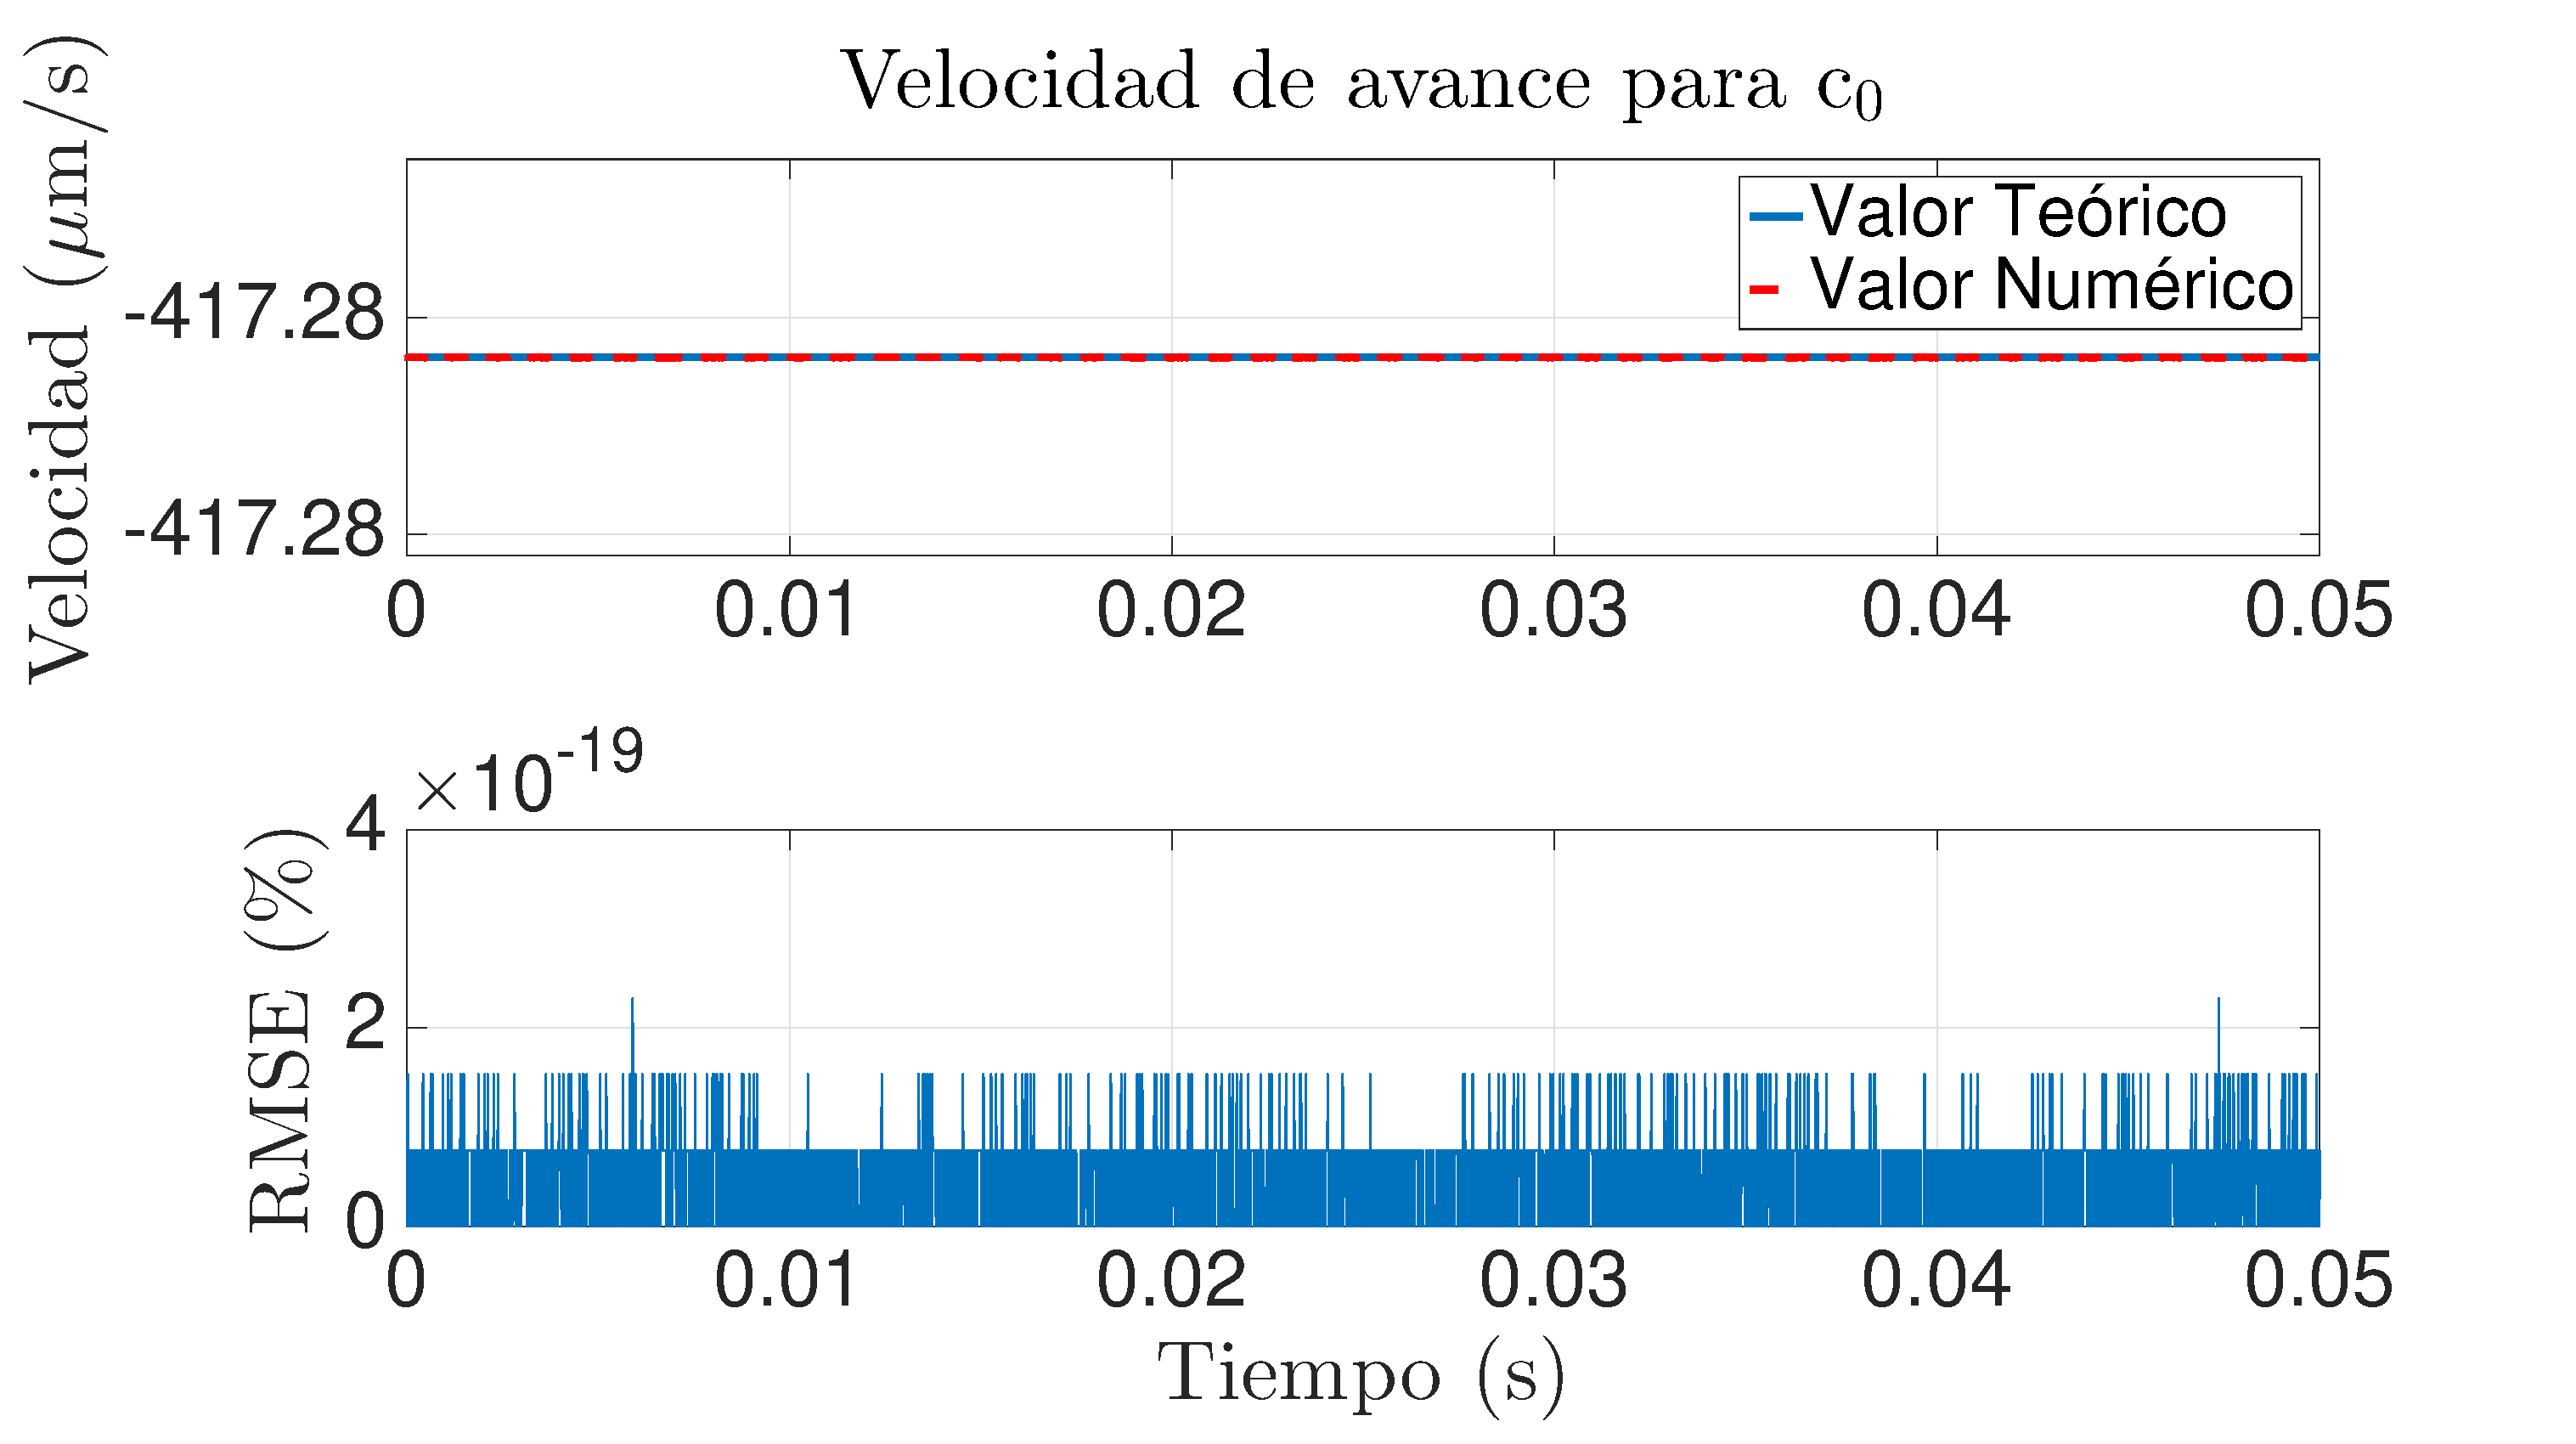
\includegraphics[width=0.45\textwidth]{Figuras/VC0}
    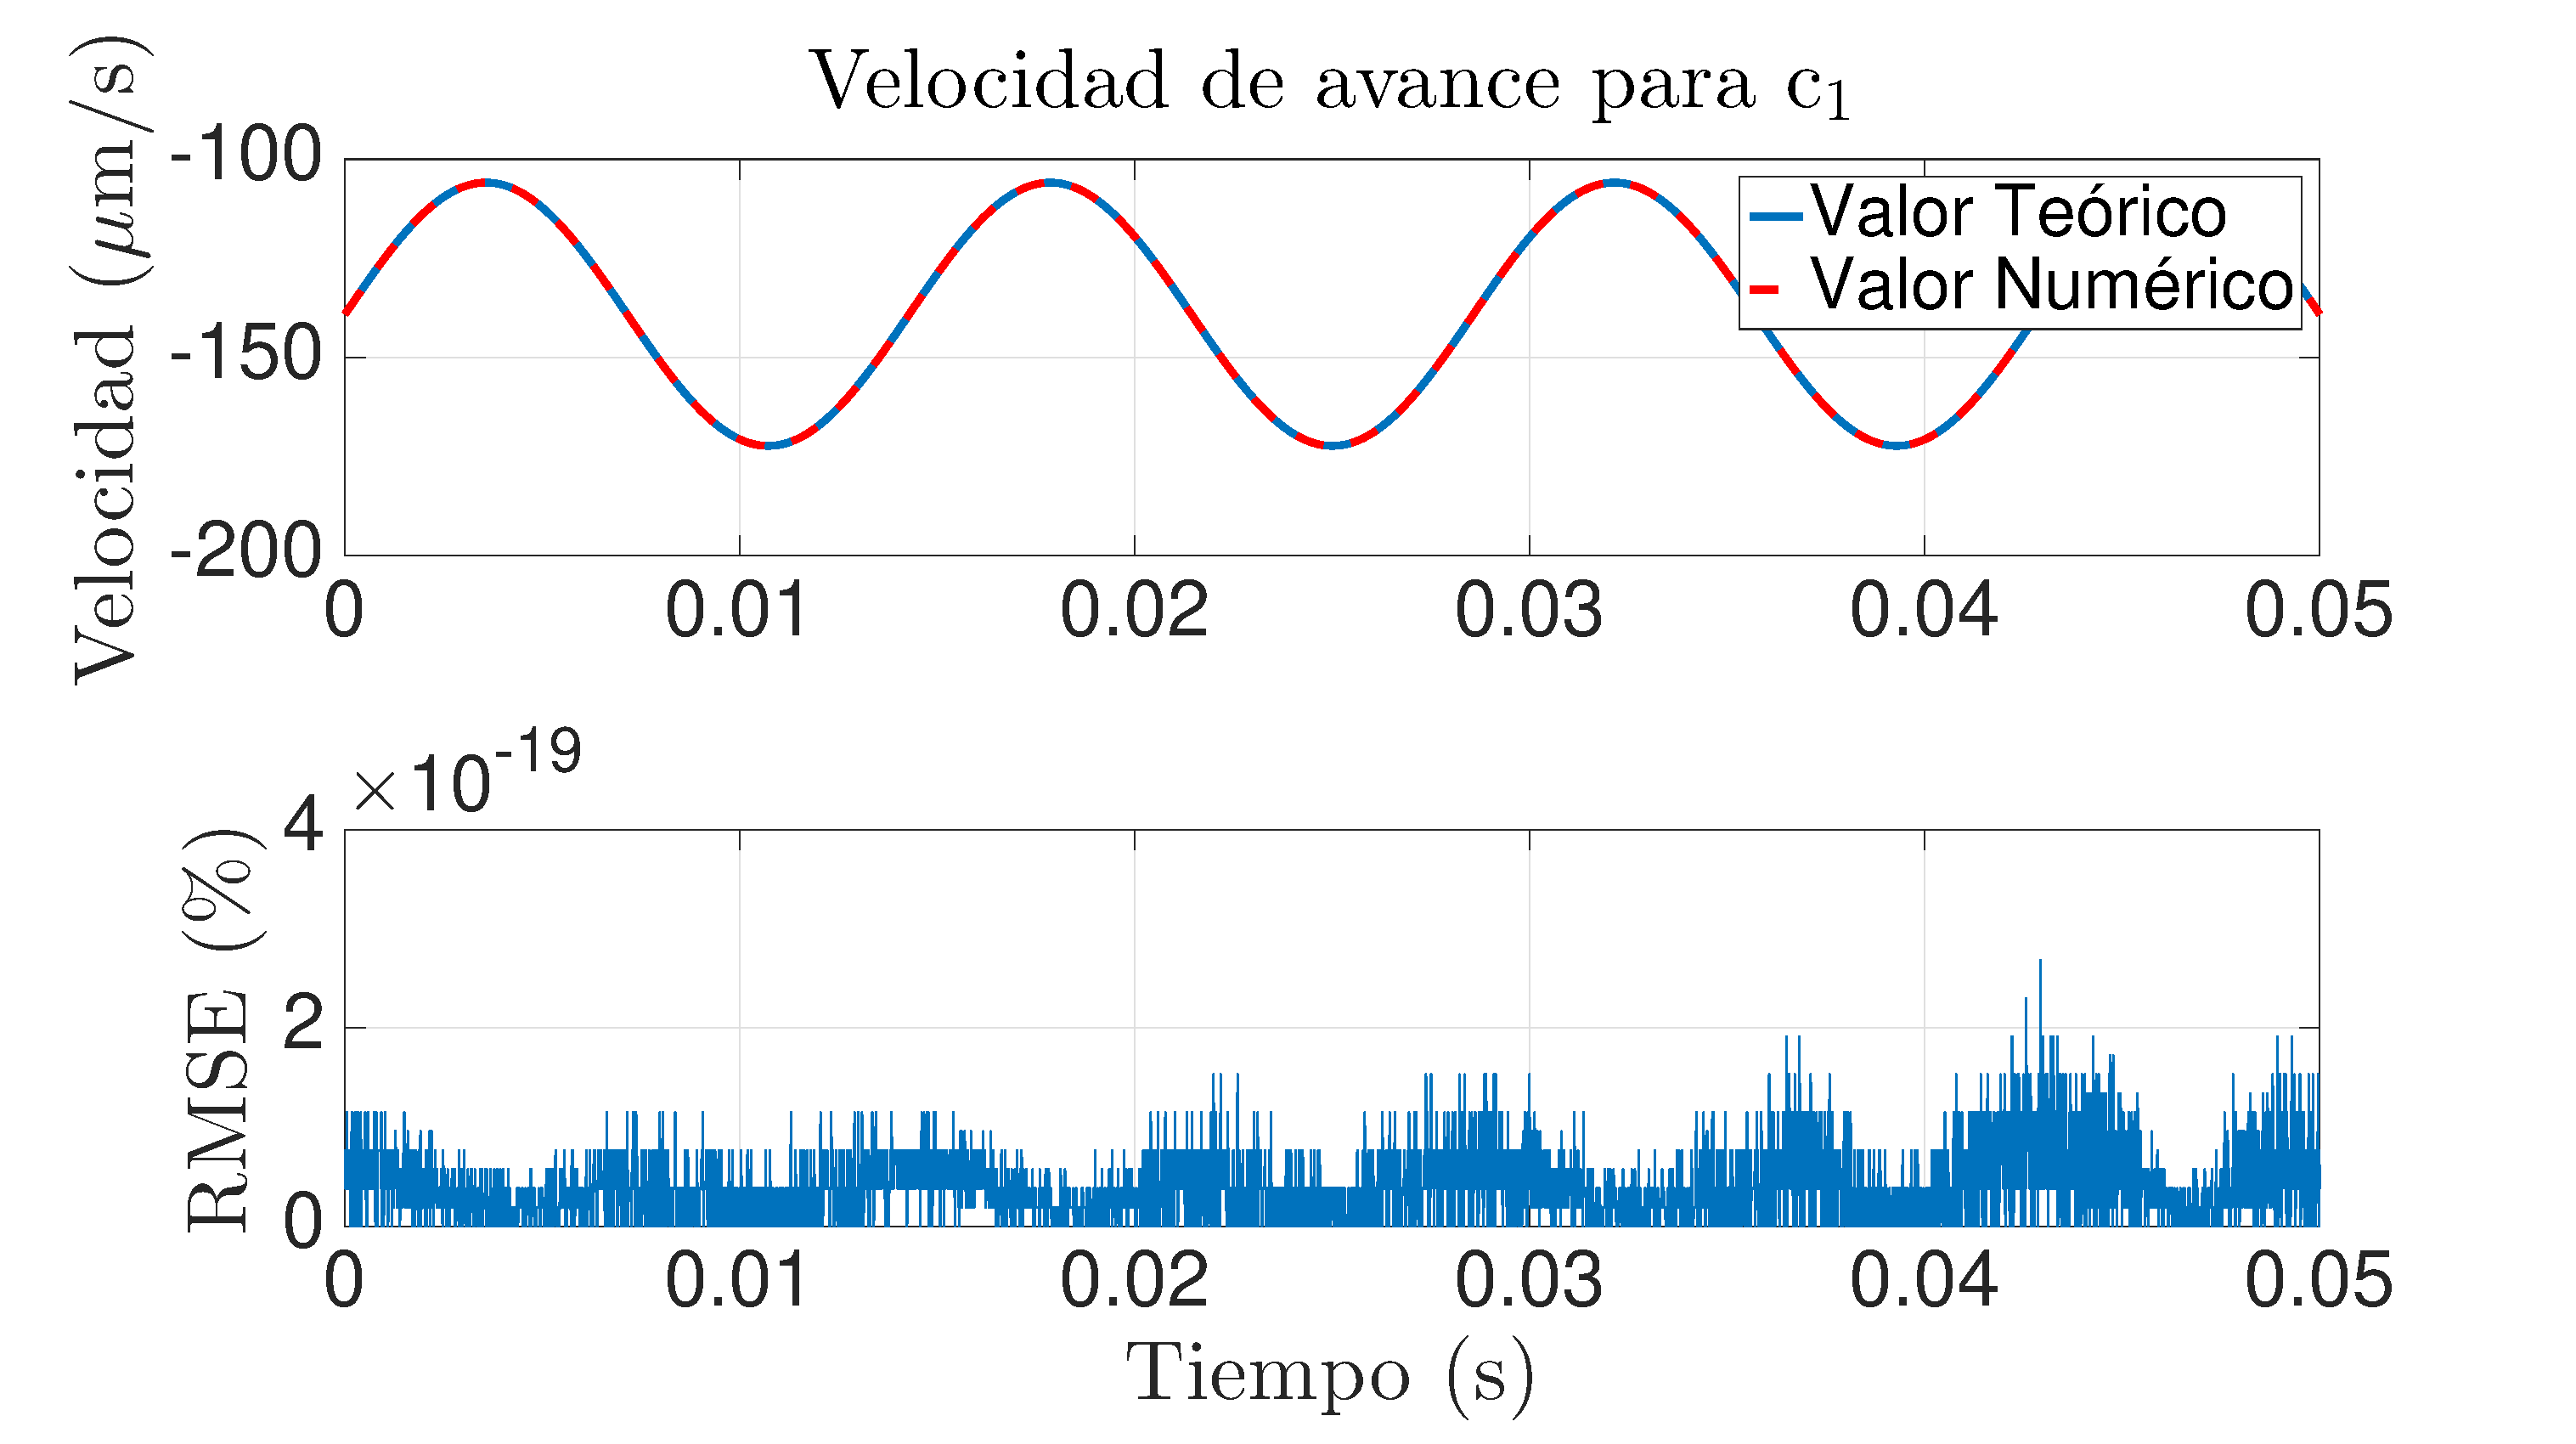
\includegraphics[width=0.45\textwidth]{Figuras/VC1}
    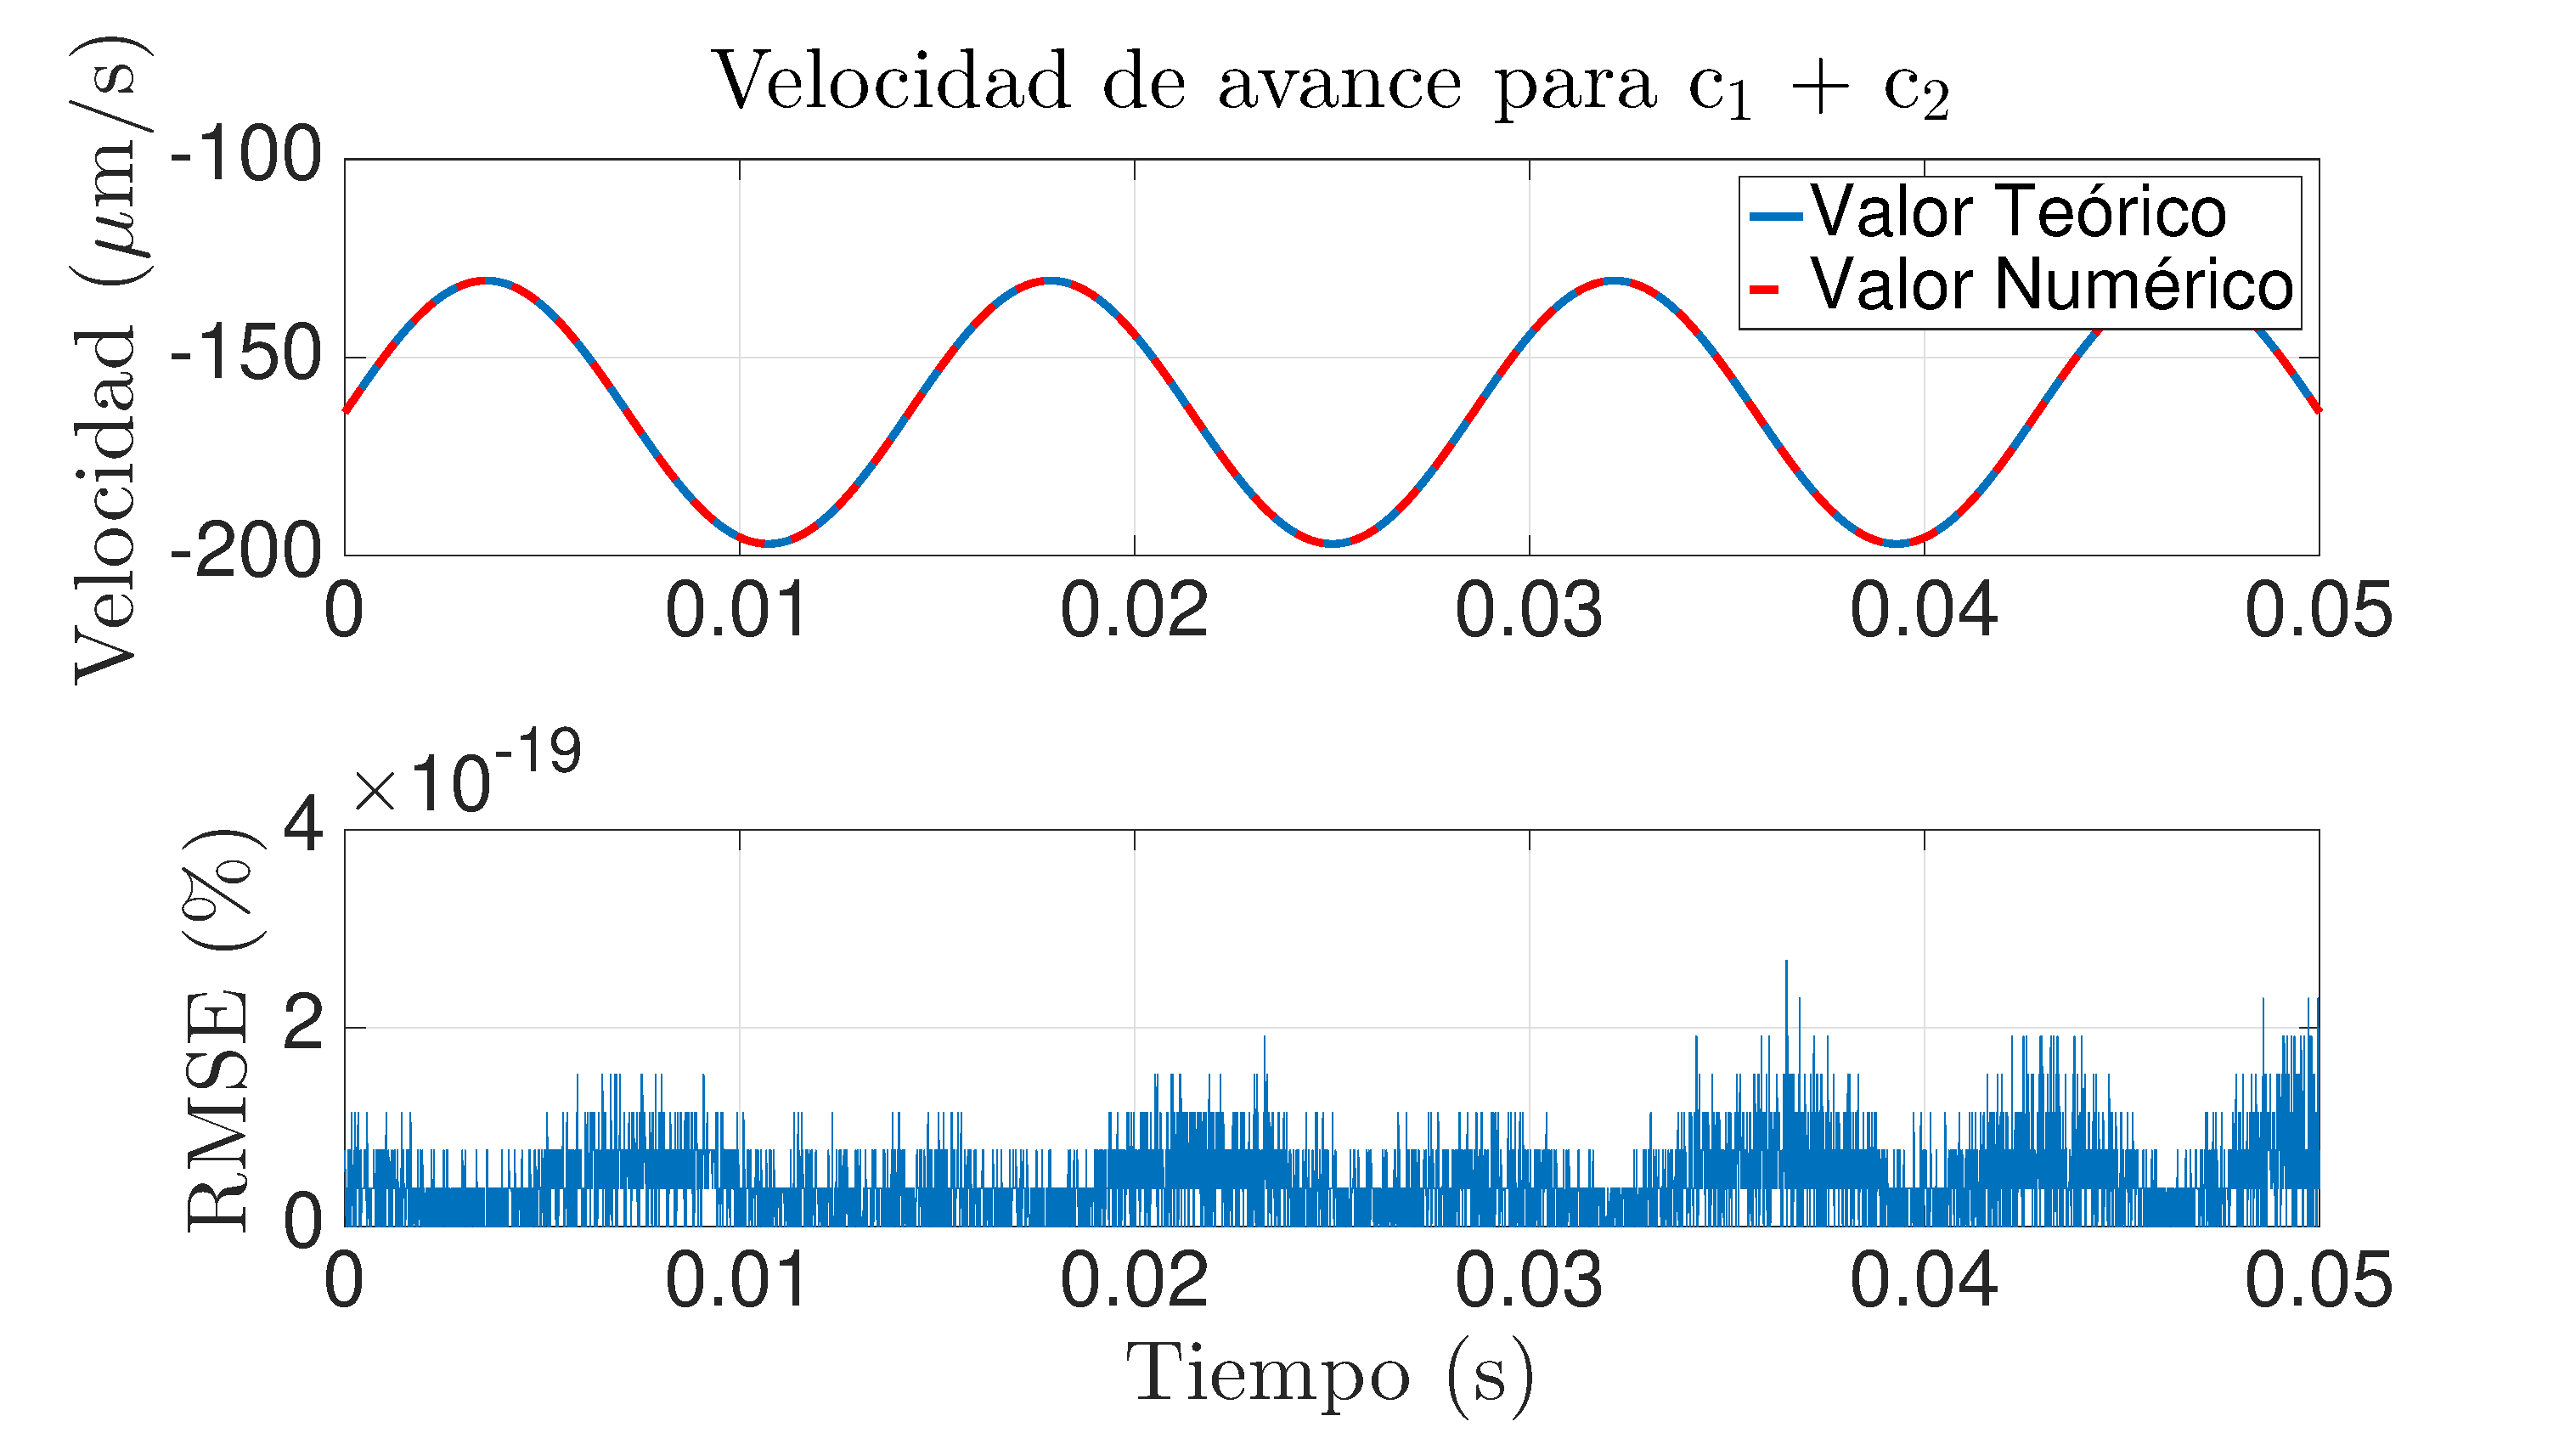
\includegraphics[width=0.5\textwidth]{Figuras/VC2}
  	\caption{Verificación algoritmo de integración numérica.}
  	\label{fig:OVVC}
\end{figure}
\newpage
%---------------------------------------
\subsection{Cálculo y análisis de velocidad de onda viajera fraccionaria} \label{sec:analisis_velocidad}
%-------------------------------------

Después de verificar que el script desarrollado es válido, proporcionando unos datos coherentes respecto a los valores teóricos. Se va a analizar la velocidad obtenida para la expresión de onda viajera indicada en (\ref{eq:flag_fish_traveling_wave_fractional}) y representadas en la Figura \ref{fig:OVF}. Siendo sus respectivas velocidades las mostradas en la Figura \ref{fig:VCF}. 
\begin{figure}[!h] %  figure placement: here, top, bottom, or page
	\vspace*{3mm}
    \centering
    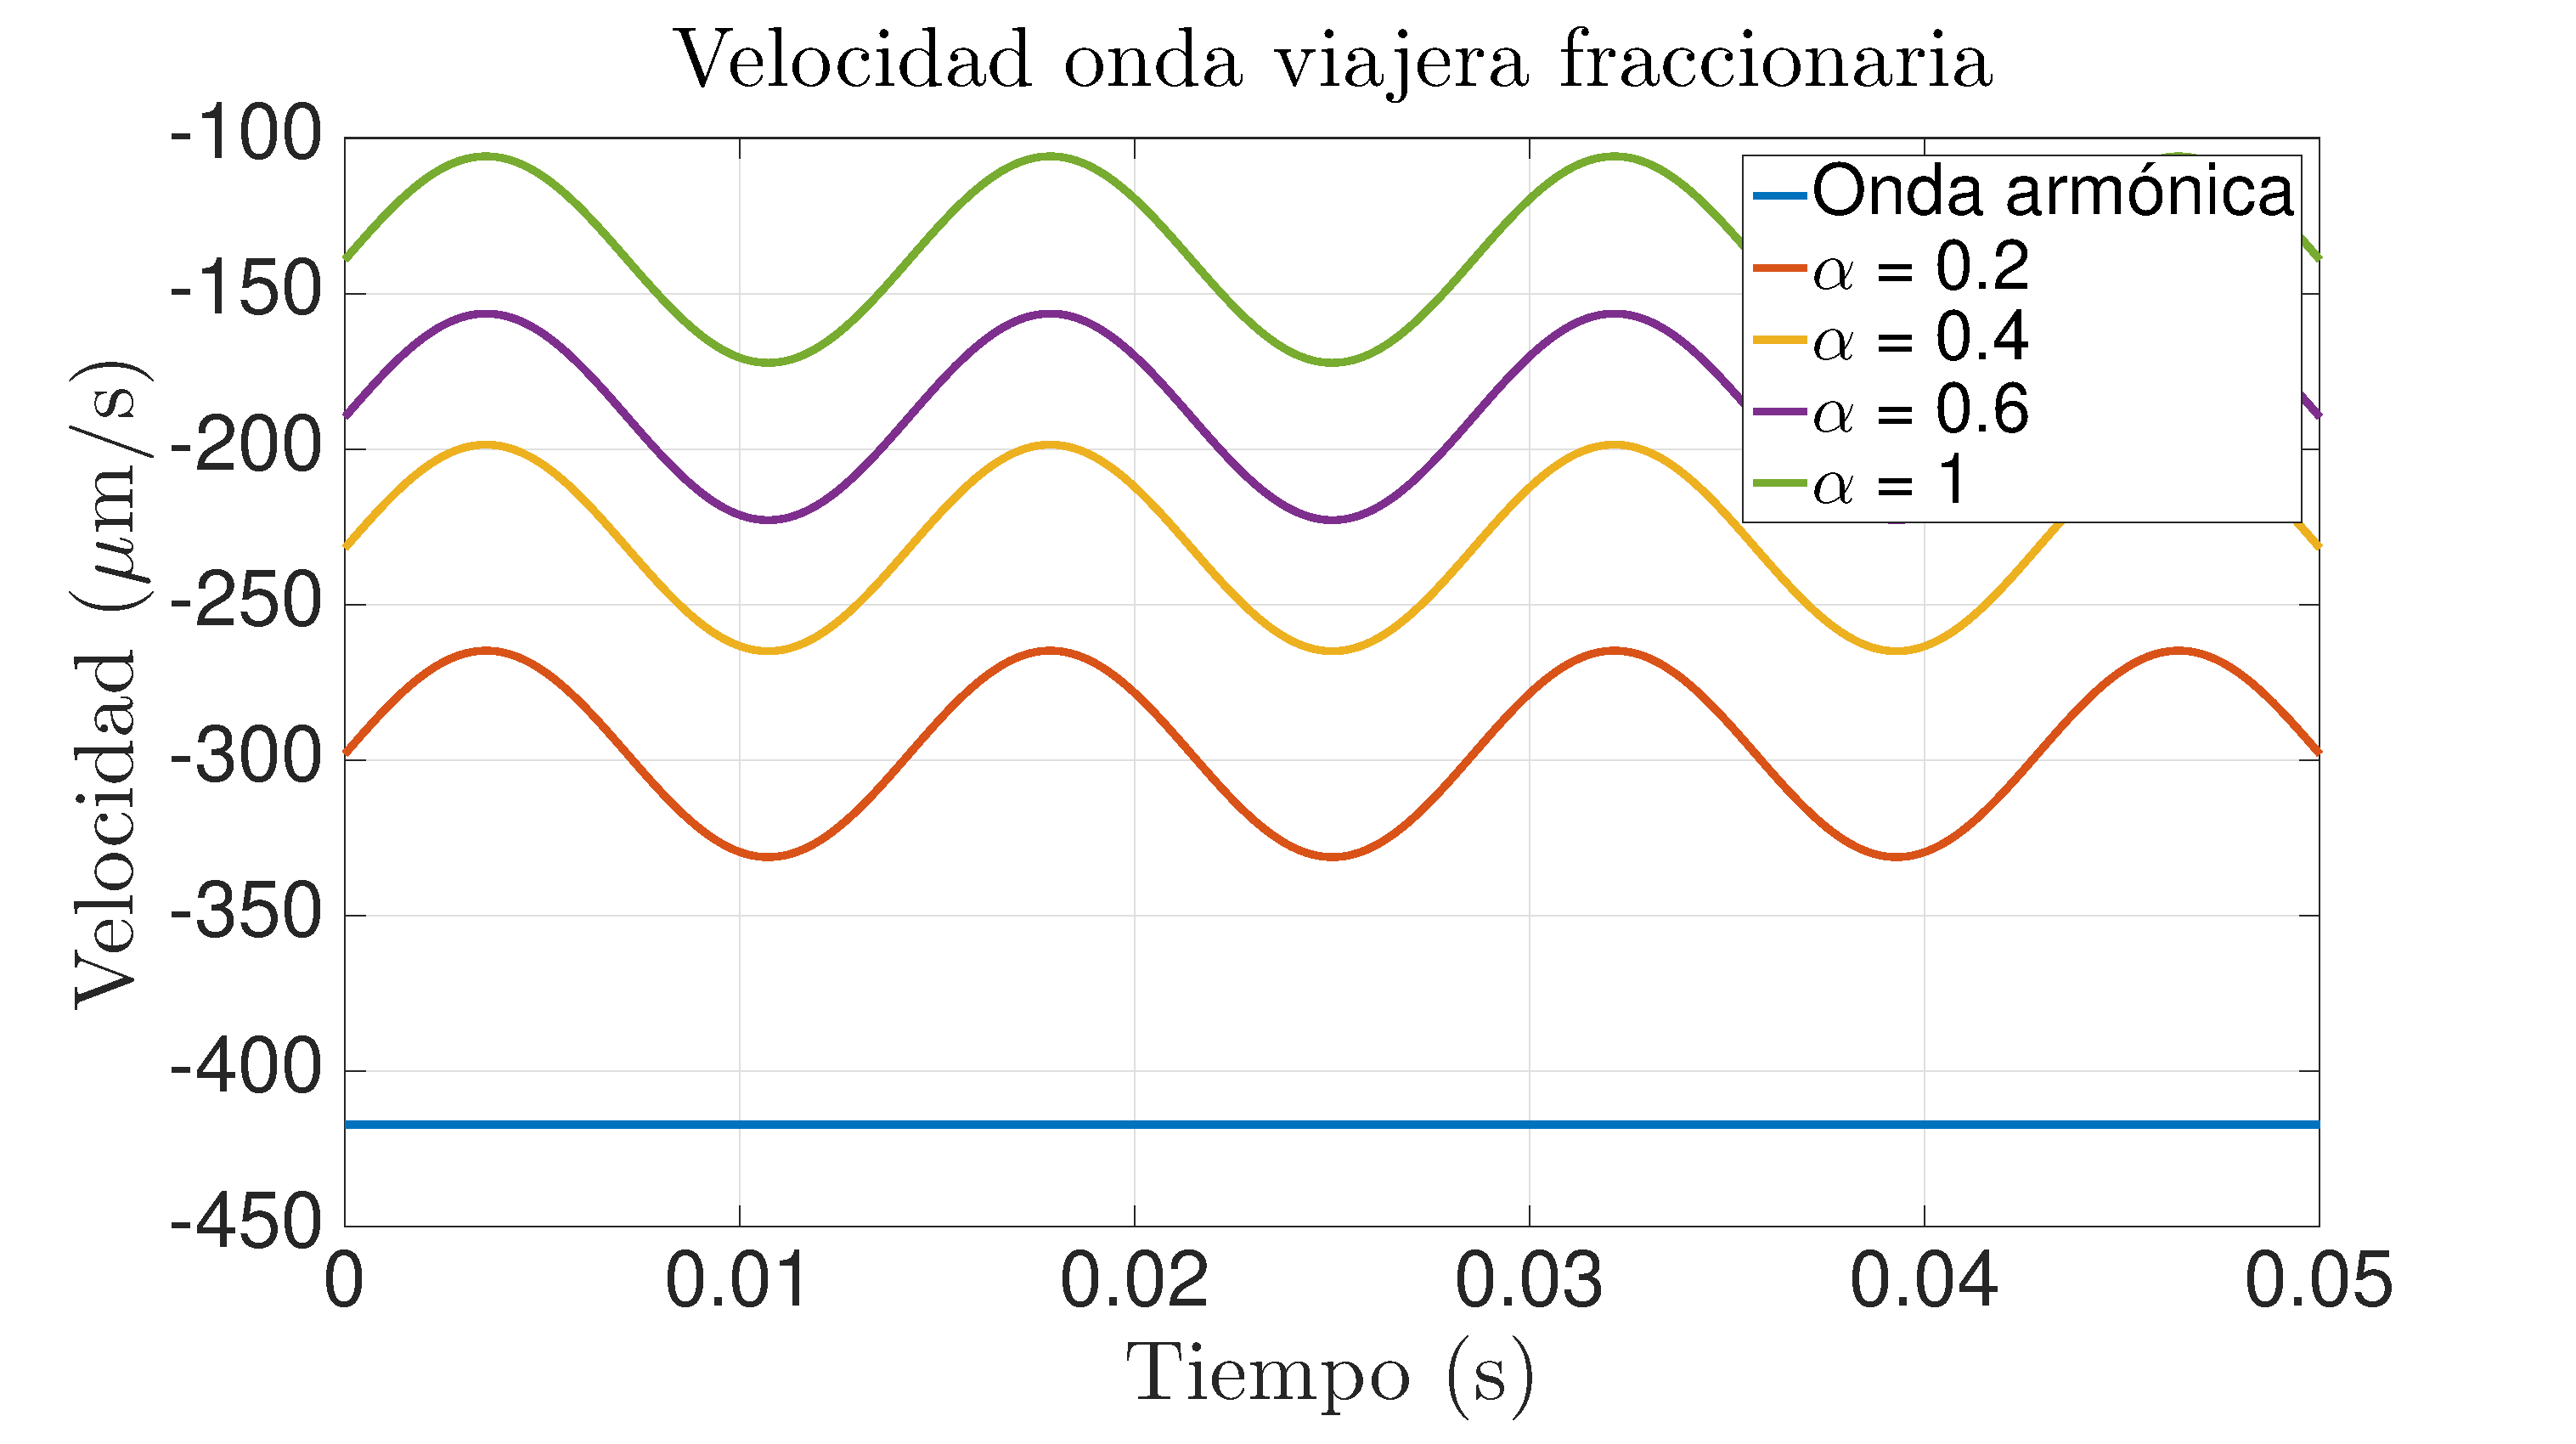
\includegraphics[width=0.85\textwidth]{Figuras/VCF}
  	\caption{Velocidad de avance onda viajera fraccionaria de pequeña señal.}
  	\label{fig:VCF}
\end{figure}

Los resultados obtenidos permite validar los afirmaciones realizadas anteriormente, es decir, la expresión de onda viajera fraccionaria proporciona una mayor fuerza de propulsión y por lo tanto velocidad de avance, ya que describe un crecimiento más rápido de las oscilaciones hasta alcanzar la amplitud máxima. Así mismo, coeficientes más bajos implican una mayor velocidad de avance, como se puede observar en la Figura, alcanzado 71.43\% de la velocidad óptima para un $\alpha$ = 0.2, en comparación al 33.33\% o 39.25\% alcanzado con la expresión \ref{eq:flag_fish_traveling_wave} con coeficiente lineal y posterior modulación, respectivamente.



















